\section{Diode}\label{dioden}
Die Diode lässt den Strom in eine Richtung passieren und in der andere Richtung sperrt sie den Stromfluss.
\begin{center}
	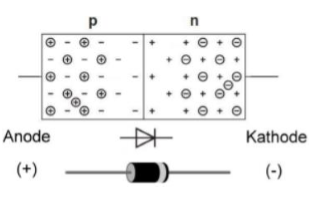
\includegraphics[width=0.4\columnwidth]{Images/diode_grafik}
\end{center}
Die Diode mit Sättigungsstrom $I_S$ und dem Emissionskoeffizient $n$ (typisch: 1.2) mit 
\[V_T(\delta = 23^\circ C) = \frac{1.38\cdot10^{-23}\frac{J}{K}\cdot (\delta + 273.15K)}{1.6\cdot10^{-19}C} = 25.5mV\]
ergibt sich die Diodenformel. Für $V_D > 200mV$ kann $-1\cdot I_S$ vernachlässigt werden:
\[
I_D(V_D) = I_S \cdot \left(e^{\frac{V_D}{n\cdot V_T}}- 1\right)
\]

\subsection{Ersatzschaltbilder}
\begin{minipage}{0.20\textwidth}
	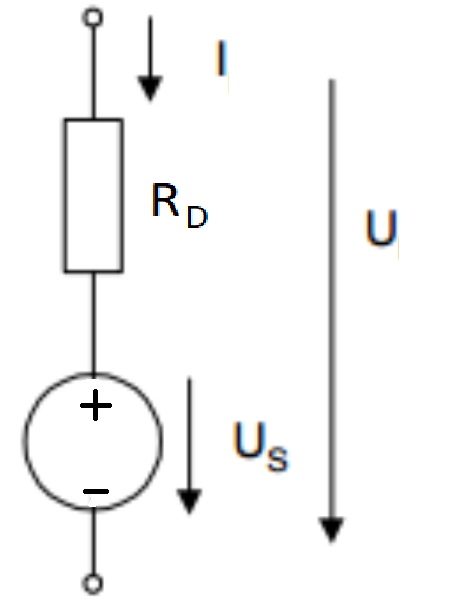
\includegraphics[width=\linewidth,keepaspectratio=true]{./Images/diode_esb}
\end{minipage}%%% to prevent a space
\begin{minipage}{0.30\textwidth}
	Um Dioden-Schaltung auszurechnen können Ersatzschaltungen am Arbeitspunkt bestimmt werden mit Sättigungsspannung $U_S \approx 0.7V$. Der Widerstand lässt sich mit $R_D = \frac{\Delta I}{\Delta V}$ beschreiben. \\
\end{minipage}

\subsection{Diodenkennlinie}
Der Innenwiderstand kann durch Ableiten von $R_D = \frac{\Delta I}{\Delta V}$ erhalten werden.\\

\textbf{Beispiel:} Widerstand bei $R(v = 0.5V) = \frac{0.5 - 0}{0^+} = \infty\Omega$ oder $R(v = 1V) = \frac{1 - 0.7}{0.3 - 0} = 1\Omega$\\
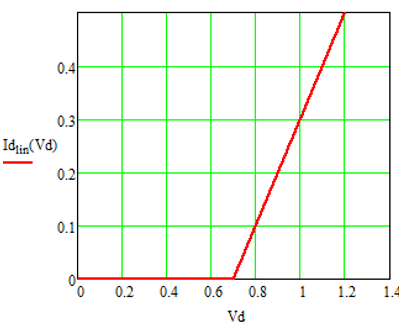
\includegraphics[width=0.4\columnwidth]{Images/diodenkennlinie}

\subsection{Temperaturverhalten}
Diodenspannung nimmt pro Grad Celsius um 2mV ab. 
\[\frac{dV}{dT} = -2\frac{mV}{K}\]
Dabei nimmt die Ausfallrate von Bauteilen um das Doppelete zu pro 10Grad.

\subsection{Spezielle Dioden}
\noindent\textbf{Schottky-Dioden} haben eine Flussspannung von ~0.3V. Der Sättigungssperrstrom $I_S$ ist aber sehr viel höher als bei Si-Dioden.~\\
\noindent\textbf{Zener-Dioden} werden vorallem für Spannungsbegrenzer und Spannungsreferenzen eingesetzt. zB um vor Überspannungen oder falsche Polung zu schützen.~\\
\noindent\textbf{Varicap} können Kapazitäten ändern und so zB Schwingkreise in Oscillatoren einstellen.~\\
\noindent\textbf{Germanium-Dioden} haben gegenüber Si-Dioden kleinere Schwellspannungen Si-Dioden 0.6..0.8V; Ge-Dioden 0.1V..0.4V. Sie sind jedoch heute nicht mehr verbreitet.



